\section{Aufbau}
\label{sec:Aufbau}
Eine Skizze der Messapparatur ist in Abbildung \ref{fig:aufbau} zu sehen.

Die Lichtquelle links oben ist eine Halogen-Lampe, das Spektrum dieser ist
im Infraroten. Die nachfolgende Linse sammelt möglichst viel Licht ein.
Der Lichtzerhacker teilt den kontinuierlichen Lichtstrahl in Pulse auf,
sodass mit dem Selektivverstärker gerade diese Frequenz verstärkt werden kann.
Für die Messergebnisse bringt dies eine Verringerung im Rauschen bei den anderen Frequenzen.

Der \enquote{Polarisator mit Goniometer} dient als Polarisator,
dessen Winkel eingestellt werden kann.
Im, dem Lichtstrahl, folgenden Elektromagneten mit Ferromagnetikum ist ein
Luftspalt, in den die Proben eingesetzt werden können.
Es gibt zu dem eine Bohrung für das Licht.

Hinter dem Elektromagneten ist ein Halter für die Interferenzfilter.
Es gibt neun Stück im Bereich von $\SI{1.06}{\micro\meter}$ bis $\SI{2.65}{\micro\meter}$.

Der \enquote{Analysator} ist feststehend und spaltet den ankommenden Lichtstrahl
in zwei mit orthogonaler Polarisation auf.
Diese werden mit zwei Photodioden detektiert.

Interessant sind die Winkel, bei denen die Differenz zwischen diesen beiden
Intensitäten verschwindet, weswegen ein Differenzverstärker verwendet wird.
Danach ist der oben erwähnte Selektivverstärker eingebaut. 
Das Ausgangssignal wird auf einem Oszilloskop dargestellt.

\begin{figure}
  \centering
  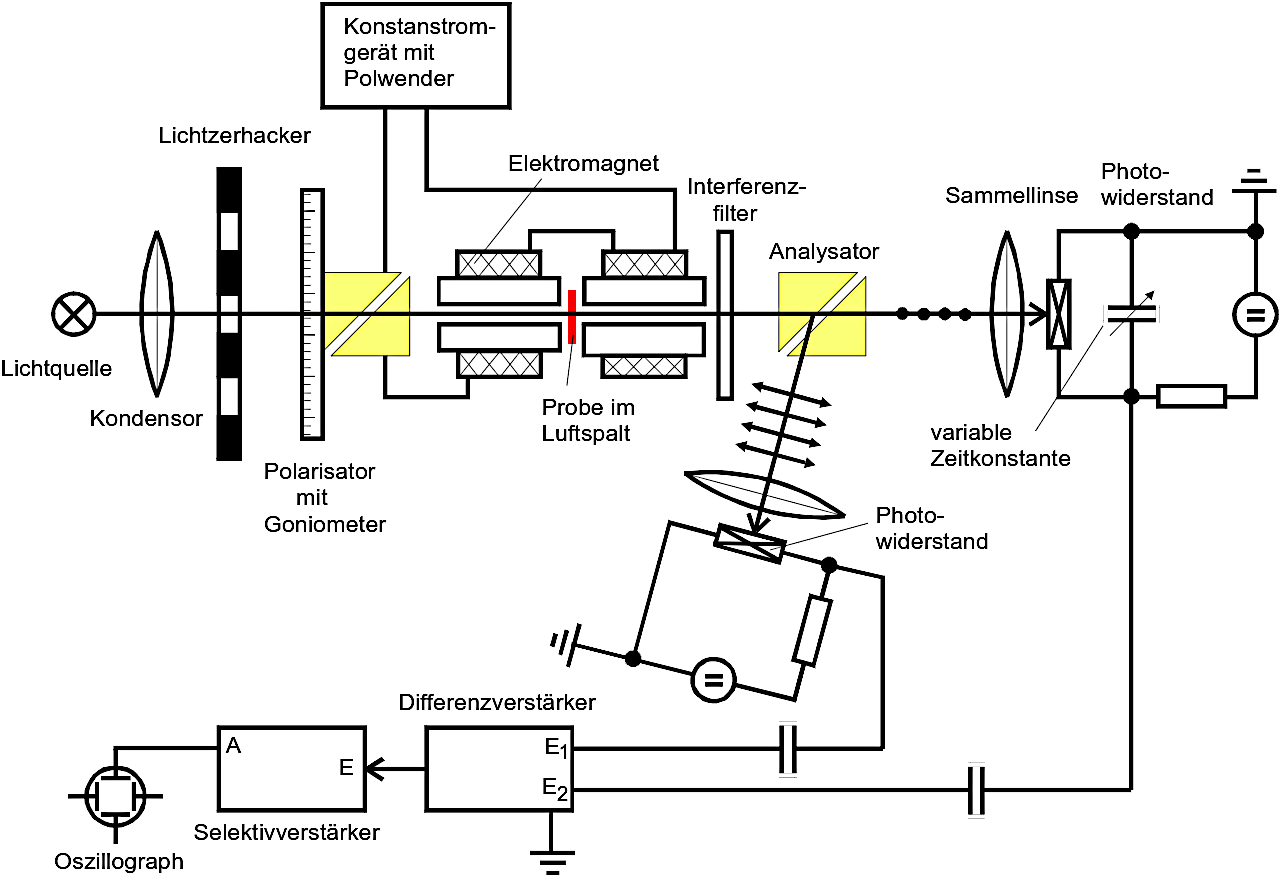
\includegraphics[width=0.9\textwidth]{images/aufbau.png}
  \caption{Skizze des Versuchsaufbaus \cite{anleitung}.}
  \label{fig:aufbau}
\end{figure}

\section{Durchführung}
\label{sec:durchfuehrung}
In der ersten Messung wird mit einer Hall-Sonde das Magnetfeld in der Spule
am Ort der Probe vermessen.

Anschließend werden die Photdioden so ausgerichtet, dass die Lichtstrahlen in
die Mitte des Sensors fallen.
Dann wird die Probe~1 eingesetzt und einer der Interferenzfilter.
An einer der Dioden ist eine Schaltung angebracht, die das Signal verzögert um
Laufzeiten auszugleichen. Hierfür ist auch der Lichtzerhacker anzustellen.

Es wird von nun an immer die Position des Polarisators gesucht,
an dem das Signal am Oszilloskop minimal ist, wobei beachtet werden muss,
dass dies alle $\SI{90}{\degree}$ geschieht.

Anschließend wird das Magnetfeld umgepolt, dafür muss erst der Strom runtergeregelt werden,
um dann die Kabel tauschen zu können. Dieses Vorgehen verhindert Influenzerscheinungen.
Die Grundmessung wird für alle Interferenzfilter und dann für Probe~2
und die Rein-Probe (Probe~0) wiederholt.
\begin{table}
  \centering
  \caption{Daten der Proben.}
  \label{tab:proben}
  \begin{tabular}{S[table-format=1.0] S[table-format=1.1] S[table-format=1.3]}
    \toprule
    {Nummer} & {$N\:/\:\SI{e18}{\centi\meter\tothe{-3}}$} & {$L\:/\:\si{\milli\meter}$} \\
    \midrule
    0 & 0   & 5.11  \\
    1 & 1.2 & 1.36  \\
    2 & 2.8 & 1.296 \\
    \bottomrule
  \end{tabular}
\end{table}
